% Options for packages loaded elsewhere
\PassOptionsToPackage{unicode}{hyperref}
\PassOptionsToPackage{hyphens}{url}
\PassOptionsToPackage{dvipsnames,svgnames,x11names}{xcolor}
%
\documentclass[
]{article}
\usepackage{amsmath,amssymb}
\usepackage{lmodern}
\usepackage{iftex}
\ifPDFTeX
  \usepackage[T1]{fontenc}
  \usepackage[utf8]{inputenc}
  \usepackage{textcomp} % provide euro and other symbols
\else % if luatex or xetex
  \usepackage{unicode-math}
  \defaultfontfeatures{Scale=MatchLowercase}
  \defaultfontfeatures[\rmfamily]{Ligatures=TeX,Scale=1}
\fi
% Use upquote if available, for straight quotes in verbatim environments
\IfFileExists{upquote.sty}{\usepackage{upquote}}{}
\IfFileExists{microtype.sty}{% use microtype if available
  \usepackage[]{microtype}
  \UseMicrotypeSet[protrusion]{basicmath} % disable protrusion for tt fonts
}{}
\makeatletter
\@ifundefined{KOMAClassName}{% if non-KOMA class
  \IfFileExists{parskip.sty}{%
    \usepackage{parskip}
  }{% else
    \setlength{\parindent}{0pt}
    \setlength{\parskip}{6pt plus 2pt minus 1pt}}
}{% if KOMA class
  \KOMAoptions{parskip=half}}
\makeatother
\usepackage{xcolor}
\usepackage[margin=1in]{geometry}
\usepackage{color}
\usepackage{fancyvrb}
\newcommand{\VerbBar}{|}
\newcommand{\VERB}{\Verb[commandchars=\\\{\}]}
\DefineVerbatimEnvironment{Highlighting}{Verbatim}{commandchars=\\\{\}}
% Add ',fontsize=\small' for more characters per line
\usepackage{framed}
\definecolor{shadecolor}{RGB}{248,248,248}
\newenvironment{Shaded}{\begin{snugshade}}{\end{snugshade}}
\newcommand{\AlertTok}[1]{\textcolor[rgb]{0.94,0.16,0.16}{#1}}
\newcommand{\AnnotationTok}[1]{\textcolor[rgb]{0.56,0.35,0.01}{\textbf{\textit{#1}}}}
\newcommand{\AttributeTok}[1]{\textcolor[rgb]{0.77,0.63,0.00}{#1}}
\newcommand{\BaseNTok}[1]{\textcolor[rgb]{0.00,0.00,0.81}{#1}}
\newcommand{\BuiltInTok}[1]{#1}
\newcommand{\CharTok}[1]{\textcolor[rgb]{0.31,0.60,0.02}{#1}}
\newcommand{\CommentTok}[1]{\textcolor[rgb]{0.56,0.35,0.01}{\textit{#1}}}
\newcommand{\CommentVarTok}[1]{\textcolor[rgb]{0.56,0.35,0.01}{\textbf{\textit{#1}}}}
\newcommand{\ConstantTok}[1]{\textcolor[rgb]{0.00,0.00,0.00}{#1}}
\newcommand{\ControlFlowTok}[1]{\textcolor[rgb]{0.13,0.29,0.53}{\textbf{#1}}}
\newcommand{\DataTypeTok}[1]{\textcolor[rgb]{0.13,0.29,0.53}{#1}}
\newcommand{\DecValTok}[1]{\textcolor[rgb]{0.00,0.00,0.81}{#1}}
\newcommand{\DocumentationTok}[1]{\textcolor[rgb]{0.56,0.35,0.01}{\textbf{\textit{#1}}}}
\newcommand{\ErrorTok}[1]{\textcolor[rgb]{0.64,0.00,0.00}{\textbf{#1}}}
\newcommand{\ExtensionTok}[1]{#1}
\newcommand{\FloatTok}[1]{\textcolor[rgb]{0.00,0.00,0.81}{#1}}
\newcommand{\FunctionTok}[1]{\textcolor[rgb]{0.00,0.00,0.00}{#1}}
\newcommand{\ImportTok}[1]{#1}
\newcommand{\InformationTok}[1]{\textcolor[rgb]{0.56,0.35,0.01}{\textbf{\textit{#1}}}}
\newcommand{\KeywordTok}[1]{\textcolor[rgb]{0.13,0.29,0.53}{\textbf{#1}}}
\newcommand{\NormalTok}[1]{#1}
\newcommand{\OperatorTok}[1]{\textcolor[rgb]{0.81,0.36,0.00}{\textbf{#1}}}
\newcommand{\OtherTok}[1]{\textcolor[rgb]{0.56,0.35,0.01}{#1}}
\newcommand{\PreprocessorTok}[1]{\textcolor[rgb]{0.56,0.35,0.01}{\textit{#1}}}
\newcommand{\RegionMarkerTok}[1]{#1}
\newcommand{\SpecialCharTok}[1]{\textcolor[rgb]{0.00,0.00,0.00}{#1}}
\newcommand{\SpecialStringTok}[1]{\textcolor[rgb]{0.31,0.60,0.02}{#1}}
\newcommand{\StringTok}[1]{\textcolor[rgb]{0.31,0.60,0.02}{#1}}
\newcommand{\VariableTok}[1]{\textcolor[rgb]{0.00,0.00,0.00}{#1}}
\newcommand{\VerbatimStringTok}[1]{\textcolor[rgb]{0.31,0.60,0.02}{#1}}
\newcommand{\WarningTok}[1]{\textcolor[rgb]{0.56,0.35,0.01}{\textbf{\textit{#1}}}}
\usepackage{graphicx}
\makeatletter
\def\maxwidth{\ifdim\Gin@nat@width>\linewidth\linewidth\else\Gin@nat@width\fi}
\def\maxheight{\ifdim\Gin@nat@height>\textheight\textheight\else\Gin@nat@height\fi}
\makeatother
% Scale images if necessary, so that they will not overflow the page
% margins by default, and it is still possible to overwrite the defaults
% using explicit options in \includegraphics[width, height, ...]{}
\setkeys{Gin}{width=\maxwidth,height=\maxheight,keepaspectratio}
% Set default figure placement to htbp
\makeatletter
\def\fps@figure{htbp}
\makeatother
\setlength{\emergencystretch}{3em} % prevent overfull lines
\providecommand{\tightlist}{%
  \setlength{\itemsep}{0pt}\setlength{\parskip}{0pt}}
\setcounter{secnumdepth}{5}
\newlength{\cslhangindent}
\setlength{\cslhangindent}{1.5em}
\newlength{\csllabelwidth}
\setlength{\csllabelwidth}{3em}
\newlength{\cslentryspacingunit} % times entry-spacing
\setlength{\cslentryspacingunit}{\parskip}
\newenvironment{CSLReferences}[2] % #1 hanging-ident, #2 entry spacing
 {% don't indent paragraphs
  \setlength{\parindent}{0pt}
  % turn on hanging indent if param 1 is 1
  \ifodd #1
  \let\oldpar\par
  \def\par{\hangindent=\cslhangindent\oldpar}
  \fi
  % set entry spacing
  \setlength{\parskip}{#2\cslentryspacingunit}
 }%
 {}
\usepackage{calc}
\newcommand{\CSLBlock}[1]{#1\hfill\break}
\newcommand{\CSLLeftMargin}[1]{\parbox[t]{\csllabelwidth}{#1}}
\newcommand{\CSLRightInline}[1]{\parbox[t]{\linewidth - \csllabelwidth}{#1}\break}
\newcommand{\CSLIndent}[1]{\hspace{\cslhangindent}#1}
\usepackage{algorithm}
\usepackage{algorithmic}
\ifLuaTeX
  \usepackage{selnolig}  % disable illegal ligatures
\fi
\IfFileExists{bookmark.sty}{\usepackage{bookmark}}{\usepackage{hyperref}}
\IfFileExists{xurl.sty}{\usepackage{xurl}}{} % add URL line breaks if available
\urlstyle{same} % disable monospaced font for URLs
\hypersetup{
  pdftitle={Respiratory Rate Determination by ECG Monitoring},
  pdfauthor={Stephen Su, 844503, COMP90072},
  colorlinks=true,
  linkcolor={Maroon},
  filecolor={Maroon},
  citecolor={Blue},
  urlcolor={blue},
  pdfcreator={LaTeX via pandoc}}

\title{Respiratory Rate Determination by ECG Monitoring}
\author{Stephen Su, 844503, COMP90072}
\date{}

\begin{document}
\maketitle

\hypertarget{introduction}{%
\section{Introduction}\label{introduction}}

\hypertarget{background}{%
\subsection{Background}\label{background}}

Pneumonia is the deadliest infectious disease to children under the age
of 5, responsible for 740,180 deaths under 5 as of 2019 (World Health
Organisation, 2022). The worsening symptoms of pneumonia can rapidly
become life-threatening for young children if not treated on time.
Nevertheless, the early stage of pneumonia with young children is often
confused with other less serious respiratory disease with similar
symptoms. On the other hand, a medical institution cannot provide
comprehensive monitoring to all its patients for all potential symptoms
of pneumonia due to limitation of resources. Thus it is of interest to
develop light-weight, non-evasive methods for detecting the most common
symptoms of pneumonia, as an early warning to serve as an indication of
a need for further medical interventions.

In a research outlined in Shamo'on et al. (2004), tachypnoea (average
respiratory rate \textgreater{} 50 per minute) is one of the critical
indicators of pneumonia in young children. However, the high volatility
of breath rate in children poses a major challenge for manual counting
that is both time-consuming and prone to error. In contrary, automated
respiratory monitoring often involves machine-measurement of
chest/abdomen movement or nasal airflow that are resource-costly and
possibly invasive such that the discomfort from wearing the equipment
might adversely affect its accuracy.

A potential solution to the problem above arises from the phenomenon of
\emph{respiratory sinus arrhythmia}, such that the instantaneous heart
rates increase with inspiration and decrease during expiration (Larsen
et al., 2010), by monitoring the periodicity of variation in the heart
rate, it may be possible to determine one's respiratory rate with a
simple, non-evasive method, such as by a pulse oximeter that is
resource-friendly. As such, this project attempts to develop an
efficient \emph{predictive} algorithm to accurately and precisely
determine respiratory rate from heart rate, as well as briefly discuss
its limitations and direction for future works.

\hypertarget{the-data}{%
\subsection{The data}\label{the-data}}

The \emph{apnea-ECG database} (Penzel et al., 2000) on \emph{PhysioNet}
(Goldberger et al., 2000) provides sufficiently large data sets of
approximately eight hours long records of electrocardiogram and
respiratory signals for eight subjects in a study for \emph{sleep
apnea}. The eight records consist of 100Hz signal from the
electrocardiogram (ECG), respiratory effort from chest/abdomen
movements, nasal airflow, and blood O\(_2\) saturation over time.

A major concern of using such data is the misalignment of objective for
the researches. Study for apnea typically involves subjects with airway
obstruction, a factor that must be considered for prior to building our
model. Under the presumption that, subjects in our data might sometimes
stop breathing, the response variable of interest should be robust from
the presence of apnea. Therefore, the model will focus on exploring the
algorithm for determining the respiratory rate from the ECG signal as a
predictor for the respiratory rate implied by chest movements, assuming
that for living humans, respiratory efforts are always present.

This study will divide records from the eight subjects into two sets:

\begin{itemize}
\tightlist
\item
  Subjects a01, a02, a03, a04 and b01 form the \emph{training set}.
\item
  Subjects c01, c02 and c03 form the \emph{test set} for evaluation.
\end{itemize}

\newpage

\hypertarget{methodologies-and-implementation}{%
\section{Methodologies and
implementation}\label{methodologies-and-implementation}}

\hypertarget{data-wrangling}{%
\subsection{Data wrangling}\label{data-wrangling}}

\hypertarget{processing-ecg-signals}{%
\subsubsection{Processing ECG signals}\label{processing-ecg-signals}}

The ECG signal does not provide the heart rate directly. Instead, it is
a time series of varying electric potential that controls the rhythm of
the contraction and relaxation of the heart muscle, with a magnitude of
approximately 0.5mV in absolute value. Such a signal is often masked by
unwanted noise, such as electric signals from pectoral muscle movement,
creating a challenge in computing heart rate from the ECG signal.

\begin{figure}

{\centering 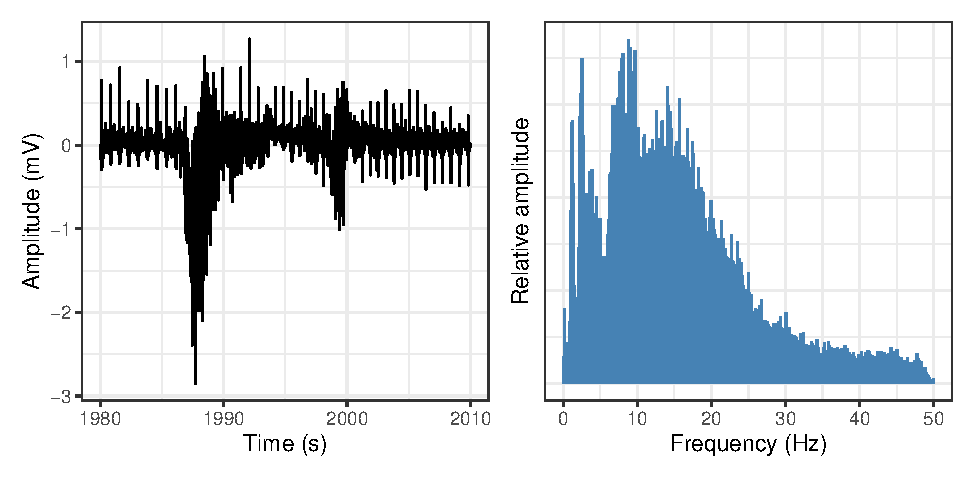
\includegraphics{report_files/figure-latex/ecg-noise-1} 

}

\caption{Left: sudden spike in noise; right: frequency spectrum of the ECG signal}\label{fig:ecg-noise}
\end{figure}

\begin{algorithm}
\caption{5-20Hz band-pass filter with fast Fourier transform}
\begin{algorithmic}[1]
\STATE Take $\mathbf{x} \in \mathbb{R}^n$ as the 100-Hz input
\STATE Obtain $\mathbf{y}$ by fast Fourier transform on $\mathbf{x}$
\FOR{$t = 1, ..., n$}
\STATE $y_t \leftarrow \sum_{k = 1}^n{x_k}\text{exp}(-2\pi i(k - 1)(t - 1) / n)$
\ENDFOR
\STATE Zero corresponding (Nyquist) frequency bins for 0-5, 20-50Hz
\FOR{$t = 1, ..., n \land (t \in (0.2n, 0.8n) \lor t > 0.95n \lor t < 0.05n)$}
\STATE $y_t \leftarrow 0 + 0i$
\ENDFOR
\STATE Obtain $\mathbf{z}$ by normalised inverse fast Fourier transform on $\mathbf{y}$
\FOR{$t = 1, ..., n$}
\STATE $z_t \leftarrow \sum_{k = 1}^n{y_k}\text{exp}(2\pi i(k - 1)(t - 1) / n) / n$
\ENDFOR
\RETURN $\text{Re}(\mathbf{z}) \in \mathbb{R}^n$ as the 100-Hz output
\end{algorithmic}
\end{algorithm}

\begin{algorithm}
\caption{R peak timestamping with phase correction}
\begin{algorithmic}[1]
\STATE Take the original $\mathbf{x} \in \mathbb{R}^n$ and the filtered $\mathbf{z} \in \mathbb{R}^n$ as the 100-Hz inputs
\STATE Set moving threshold $\mathbf{b}$ as half of rolling maximum
\STATE $(b_t | t = 1, ..., 100) \leftarrow (+\infty)_{\times 100}$
\FOR{$t = 101, ..., n$}
\STATE $b_t \leftarrow \frac{1}{2}\text{max}\{z_{t - 100}, ..., z_t\}$
\ENDFOR
\STATE Create thresholding indicator $\boldsymbol{\iota^{(1)}}$
\FOR{$t = 1, ..., n$}
\STATE $\iota^{(1)}_t \leftarrow I(z_t > \text{max}\{b_t, F^{-1}_{Z}(0.95)\})$
\ENDFOR
\STATE Create concave-peak indicator $\boldsymbol{\iota^{(2)}}$
\FOR{$t = 1, n$}
\STATE $\iota^{(2)}_t \leftarrow 0$
\ENDFOR
\FOR{$t = 2, ..., n - 1$}
\STATE $\iota^{(2)}_t \leftarrow I[I(z_{t + 1} - z_t > 0) - I(z_t - z_{t - 1} > 0) = -1]$
\ENDFOR
\STATE Preliminary timestamps for R peak $\mathbf{p} \leftarrow (t = 1, ..., n | \iota^{(1)}_t \land \iota^{(2)}_t \text{ is True})$
\STATE Remove abnormal timestamps in $\mathbf{p}$ with R-R intervals of < 300ms
\STATE Correct phase-shifts caused by fast Fourier transform
\FOR{$t \in \{\mathbf{p}\}$}
\STATE $p | p = t \leftarrow \text{argmax}_{i = t - 4, ..., t, ..., t + 4} x_i$
\ENDFOR
\RETURN $\mathbf{p}$ the timestamps of the R peak
\end{algorithmic}
\end{algorithm}

\begin{algorithm}
\caption{Deriving instantaneous heart rates from R peak timestamps}
\begin{algorithmic}[1]
\STATE Take $\mathbf{p}$ the timestamps of the R peak as the input, and $\nu$ as an argument for the frequency unit of $\mathbf{p}$
\STATE $m \leftarrow \text{dim}(\mathbf{p})$ dimension of $\mathbf{p}$
\STATE Compute the R-R intervals $\mathbf{d}$
\STATE $(d_t | t = 1, ..., p_1) \leftarrow (\text{NA})_{\times p_1}$
\STATE $(d_t | t = p_1 + 1, ..., p_{m}) \leftarrow ((p_2 - p_1)_{\times (p_2 - p_1)}, (p_3 - p_2)_{\times (p_3 - p_2)}, ..., (p_{m} - p_{m - 1})_{\times (p_{m} - p_{m - 1})})^\top$
\STATE Convert R-R intervals into heart rates per minute $\mathbf{h}$
\STATE $\mathbf{h} \leftarrow 60 \cdot \nu / \mathbf{d}$
\RETURN $\mathbf{h}$ the heart rates per minute at frequency $\nu$
\end{algorithmic}
\end{algorithm}

\begin{algorithm}
\caption{Smoothing spline crossing for counting cycles of nonstationary pseudosinusoidal oscillations, for varying heart rates/chest movements}
\begin{algorithmic}[1]
\STATE Take a time series vector $\mathbf{a}$ at any frequency, and the optional argument $\lambda$ the regularisation parameter
\STATE $\mathbf{t} \leftarrow (1, ..., \text{dim}(\mathbf{a}))^\top$ as the indexing vector
\STATE Construct B-spline bases $\mathbf{B}$ derived from natural cubic spline bases about all possible knots of $\mathbf{t}$
\STATE Penalty matrix $\boldsymbol{\Omega} \leftarrow \{\omega_{jk} = \int_T {B_j^{''}(s)B_k^{''}(s)}ds | B_j(t_i) = (\mathbf{B})_{ij}\}$
\IF{argument $\lambda$ is missing}
\STATE $\lambda \leftarrow \text{argmin}_{\lambda > 0} (1 - \text{tr}(\mathbf{B}(\mathbf{B}^\top\mathbf{B} + \lambda\boldsymbol{\Omega})^{-1}\mathbf{B}^\top) / \text{dim}(\mathbf{a}))^{-2}||(\mathbf{I} - \mathbf{B}(\mathbf{B}^\top\mathbf{B} + \lambda\boldsymbol{\Omega})^{-1}\mathbf{B}^\top)\mathbf{a}||^2$
\ENDIF
\STATE $\mathbf{\hat{a}} \leftarrow \mathbf{B}(\mathbf{B}^\top\mathbf{B} + \lambda\boldsymbol{\Omega})^{-1}\mathbf{B}^\top\mathbf{a}$
\STATE Count the number of times the curves $(\mathbf{t}, \mathbf{a})$ and $(\mathbf{t}, \mathbf{\hat{a}})$ cross (equivalent to zero-crossing for $(\mathbf{t}, \mathbf{a} - \mathbf{\hat{a}})$)
\RETURN half of the count obtained above as the approximated cycles
\end{algorithmic}
\end{algorithm}

\begin{algorithm}
\caption{Deriving breath rate from heart rate based on chest movements}
\begin{algorithmic}[1]
\STATE Take $\mathbf{h}$ the heart rates per minute and $\mathbf{c}$ the chest movements signal (either at 100Hz or down-sampled) where both time series have aligned indices and identical frequency; and optional argument $\lambda_\text{opt}$ (only in model evaluation with test data)
\STATE For both $\mathbf{h}$ and $\mathbf{c}$, remove elements of index where $c_t = \text{NA}$
\FOR{each record of all the subjects}
\STATE Partition each of $\mathbf{h}$ and $\mathbf{c}$ into segments of 60-second data
\ENDFOR
\STATE Drop the remainder (last segment), which is less than 60 seconds
\IF{$\mathbf{h}$ and $\mathbf{c}$ for more than one subject is input}
\STATE Bind $\mathbf{h}$ and $\mathbf{c}$ of all subjects together
\ENDIF
\FOR{each 60-second segment of $\mathbf{c}$}
\STATE Pass each minute of $\mathbf{c}$ into Algorithm 4 (the smoothing spline crossing, without specifying $\lambda$) to compute the true rate of breath based on chest movements, and output $\rightarrow \mathbf{r}$
\ENDFOR
\IF{argument $\lambda_\text{opt}$ is missing}
\STATE $\lambda_\text{opt} \leftarrow \text{argmin}_{\lambda > 0} ||\mathbf{r} - \hat{f}(\mathbf{h}; \lambda)||^2$ where $\hat{f}$ is the Algorithm 4: applied on each minute of $\mathbf{h}$ given $\lambda$
\ENDIF
\STATE $\hat{\lambda}_\text{opt} \leftarrow \lambda_\text{opt}$: if its value is obtained by Step 14 $\hat{\lambda}_\text{opt}$ is the estimate of $\lambda_\text{opt}$ derived from the training data; otherwise, if $\lambda_\text{opt}$ is passed as an argument, then the purpose of this algorithm is model testing
\FOR{each 60-second segment of $\mathbf{h}$}
\STATE Pass each minute of $\mathbf{h}$ into Algorithm 4 (with argument of $\lambda = \hat{\lambda}_\text{opt}$) to compute the derived rate of breath from heart rate, and output $\rightarrow \mathbf{\hat{r}}$ which is the model's estimate of $\mathbf{r}$: the chest rate of breath
\ENDFOR
\RETURN data matrix $(\mathbf{r}, \mathbf{\hat{r}})$, a bi-variate time series (minutely), $\mathbf{r} :=$ "count of breaths by chest movements (observations)" and $\mathbf{\hat{r}} :=$ "number of breaths derived by cardio-activities of that minute (fitted values)", and most importantly $\hat{\lambda}_\text{opt}$ the trained parameter for our final model!
\end{algorithmic}
\end{algorithm}

\newpage

\hypertarget{appendix-workflow-code-and-output}{%
\section{Appendix: workflow, code and
output}\label{appendix-workflow-code-and-output}}

\hypertarget{source-code}{%
\subsection{Source code}\label{source-code}}

The source codes for the functions used in the workflow are in the
\texttt{.R} files at
\href{https://github.com/szmsu2011/comp90072/blob/main/R}{/R}.

\hypertarget{data-wrangling-and-signal-processing}{%
\subsection{Data wrangling and signal
processing}\label{data-wrangling-and-signal-processing}}

\begin{Shaded}
\begin{Highlighting}[]
\NormalTok{training\_set }\OtherTok{\textless{}{-}} \FunctionTok{c}\NormalTok{(}\StringTok{"a01"}\NormalTok{, }\StringTok{"a02"}\NormalTok{, }\StringTok{"a03"}\NormalTok{, }\StringTok{"a04"}\NormalTok{, }\StringTok{"b01"}\NormalTok{)}
\NormalTok{test\_set }\OtherTok{\textless{}{-}} \FunctionTok{c}\NormalTok{(}\StringTok{"c01"}\NormalTok{, }\StringTok{"c02"}\NormalTok{, }\StringTok{"c03"}\NormalTok{)}
\NormalTok{hr }\OtherTok{\textless{}{-}} \FunctionTok{fuse\_data}\NormalTok{(}\FunctionTok{map}\NormalTok{(}
  \FunctionTok{sprintf}\NormalTok{(}\StringTok{"../data{-}bin/\%s.dat"}\NormalTok{, training\_set),}
  \ControlFlowTok{function}\NormalTok{(ecg\_file) \{}
\NormalTok{    ecg\_file }\SpecialCharTok{|\textgreater{}}
      \FunctionTok{read\_ecg}\NormalTok{() }\SpecialCharTok{|\textgreater{}}
      \FunctionTok{find\_r\_peaks}\NormalTok{() }\SpecialCharTok{|\textgreater{}}
      \FunctionTok{frequency}\NormalTok{() }\SpecialCharTok{|\textgreater{}}
      \FunctionTok{down\_sample}\NormalTok{()}
\NormalTok{  \}}
\NormalTok{))}
\NormalTok{resp }\OtherTok{\textless{}{-}} \FunctionTok{fuse\_data}\NormalTok{(}\FunctionTok{map}\NormalTok{(}
  \FunctionTok{sprintf}\NormalTok{(}\StringTok{"../data{-}bin/\%sr.dat"}\NormalTok{, training\_set),}
  \ControlFlowTok{function}\NormalTok{(resp\_file) }\FunctionTok{down\_sample}\NormalTok{(}\FunctionTok{read\_resp}\NormalTok{(resp\_file))}
\NormalTok{))}
\NormalTok{hr\_test }\OtherTok{\textless{}{-}} \FunctionTok{fuse\_data}\NormalTok{(}\FunctionTok{map}\NormalTok{(}
  \FunctionTok{sprintf}\NormalTok{(}\StringTok{"../data{-}bin/\%s.dat"}\NormalTok{, test\_set),}
  \ControlFlowTok{function}\NormalTok{(ecg\_file) \{}
\NormalTok{    ecg\_file }\SpecialCharTok{|\textgreater{}}
      \FunctionTok{read\_ecg}\NormalTok{() }\SpecialCharTok{|\textgreater{}}
      \FunctionTok{find\_r\_peaks}\NormalTok{() }\SpecialCharTok{|\textgreater{}}
      \FunctionTok{frequency}\NormalTok{() }\SpecialCharTok{|\textgreater{}}
      \FunctionTok{down\_sample}\NormalTok{()}
\NormalTok{  \}}
\NormalTok{))}
\NormalTok{resp\_test }\OtherTok{\textless{}{-}} \FunctionTok{fuse\_data}\NormalTok{(}\FunctionTok{map}\NormalTok{(}
  \FunctionTok{sprintf}\NormalTok{(}\StringTok{"../data{-}bin/\%sr.dat"}\NormalTok{, test\_set),}
  \ControlFlowTok{function}\NormalTok{(resp\_file) }\FunctionTok{down\_sample}\NormalTok{(}\FunctionTok{read\_resp}\NormalTok{(resp\_file))}
\NormalTok{))}
\FunctionTok{write\_rds}\NormalTok{(hr, }\StringTok{"../R/hr.rds"}\NormalTok{)}
\FunctionTok{write\_rds}\NormalTok{(resp, }\StringTok{"../R/resp.rds"}\NormalTok{)}
\FunctionTok{write\_rds}\NormalTok{(hr\_test, }\StringTok{"../R/hr{-}test.rds"}\NormalTok{)}
\FunctionTok{write\_rds}\NormalTok{(resp\_test, }\StringTok{"../R/resp{-}test.rds"}\NormalTok{)}
\end{Highlighting}
\end{Shaded}

\hypertarget{model-training}{%
\subsection{Model training}\label{model-training}}

\begin{Shaded}
\begin{Highlighting}[]
\NormalTok{hr }\OtherTok{\textless{}{-}} \FunctionTok{read\_rds}\NormalTok{(}\StringTok{"../R/hr.rds"}\NormalTok{)}
\NormalTok{resp }\OtherTok{\textless{}{-}} \FunctionTok{read\_rds}\NormalTok{(}\StringTok{"../R/resp.rds"}\NormalTok{)}
\NormalTok{resp\_df }\OtherTok{\textless{}{-}} \FunctionTok{resp\_dataset}\NormalTok{(hr, resp)}
\end{Highlighting}
\end{Shaded}

\begin{verbatim}
#>   opt_lambda 
#> 1.571851e-06
\end{verbatim}

\begin{center}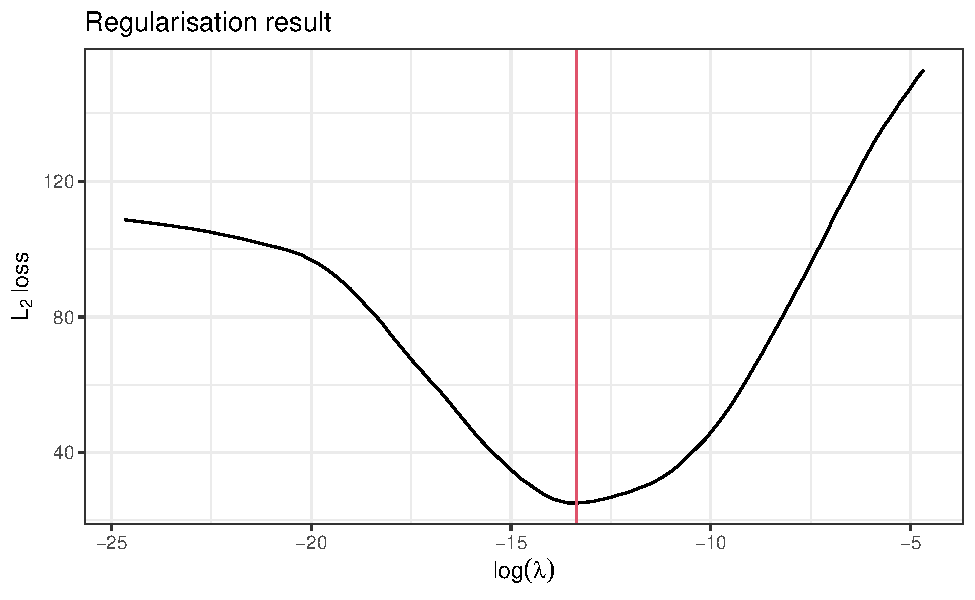
\includegraphics{report_files/figure-latex/train-1} \end{center}

\begin{Shaded}
\begin{Highlighting}[]
\NormalTok{resp\_df}
\end{Highlighting}
\end{Shaded}

\begin{verbatim}
#> # A tibble: 2,526 x 2
#>    breath_chest breath_ecg
#>           <dbl>      <dbl>
#>  1         19.5       15  
#>  2         22.5       16  
#>  3         23.5       17.5
#>  4         20.5       18  
#>  5         20.5       18  
#>  6         23         15  
#>  7         16         18  
#>  8         20         21.5
#>  9         20         17.5
#> 10         18         16.5
#> # i 2,516 more rows
\end{verbatim}

\begin{Shaded}
\begin{Highlighting}[]
\FunctionTok{summary}\NormalTok{(resp\_df)}
\end{Highlighting}
\end{Shaded}

\begin{verbatim}
#>   breath_chest     breath_ecg   
#>  Min.   : 5.50   Min.   :11.50  
#>  1st Qu.:15.00   1st Qu.:17.50  
#>  Median :18.50   Median :19.00  
#>  Mean   :18.46   Mean   :18.96  
#>  3rd Qu.:21.38   3rd Qu.:20.50  
#>  Max.   :29.00   Max.   :26.50
\end{verbatim}

\hypertarget{model-diagnostics}{%
\subsection{Model diagnostics}\label{model-diagnostics}}

\begin{Shaded}
\begin{Highlighting}[]
\FunctionTok{c}\NormalTok{(}\StringTok{"R{-}F cor"} \OtherTok{=} \FunctionTok{with}\NormalTok{(resp\_df, }\FunctionTok{cor}\NormalTok{(breath\_chest }\SpecialCharTok{{-}}\NormalTok{ breath\_ecg, breath\_ecg)))}
\end{Highlighting}
\end{Shaded}

\begin{verbatim}
#>    R-F cor 
#> -0.3976376
\end{verbatim}

\begin{Shaded}
\begin{Highlighting}[]
\NormalTok{test }\OtherTok{\textless{}{-}} \FunctionTok{lm}\NormalTok{(breath\_chest }\SpecialCharTok{\textasciitilde{}} \DecValTok{0} \SpecialCharTok{+}\NormalTok{ breath\_ecg, resp\_df)}
\FunctionTok{c}\NormalTok{(}\StringTok{"p{-}value"} \OtherTok{=} \FunctionTok{unname}\NormalTok{(}\FunctionTok{pchisq}\NormalTok{(}
  \FunctionTok{sum}\NormalTok{(resp\_df}\SpecialCharTok{$}\NormalTok{breath\_ecg}\SpecialCharTok{\^{}}\DecValTok{2}\NormalTok{) }\SpecialCharTok{*}\NormalTok{ (}\FunctionTok{coef}\NormalTok{(test) }\SpecialCharTok{{-}} \DecValTok{1}\NormalTok{)}\SpecialCharTok{\^{}}\DecValTok{2} \SpecialCharTok{*}
\NormalTok{    (}\FunctionTok{nrow}\NormalTok{(resp\_df) }\SpecialCharTok{{-}} \DecValTok{1}\NormalTok{) }\SpecialCharTok{/} \FunctionTok{sum}\NormalTok{(}\FunctionTok{residuals}\NormalTok{(test)}\SpecialCharTok{\^{}}\DecValTok{2}\NormalTok{), }\DecValTok{1}\NormalTok{,}
  \AttributeTok{lower.tail =} \ConstantTok{FALSE}
\NormalTok{)))}
\end{Highlighting}
\end{Shaded}

\begin{verbatim}
#>      p-value 
#> 2.983174e-13
\end{verbatim}

\begin{Shaded}
\begin{Highlighting}[]
\FunctionTok{confint}\NormalTok{(test)}
\end{Highlighting}
\end{Shaded}

\begin{verbatim}
#>                2.5 %    97.5 %
#> breath_ecg 0.9521173 0.9724053
\end{verbatim}

\hypertarget{model-evaluation}{%
\subsection{Model evaluation}\label{model-evaluation}}

\begin{Shaded}
\begin{Highlighting}[]
\NormalTok{hr\_test }\OtherTok{\textless{}{-}} \FunctionTok{read\_rds}\NormalTok{(}\StringTok{"../R/hr{-}test.rds"}\NormalTok{)}
\NormalTok{resp\_test }\OtherTok{\textless{}{-}} \FunctionTok{read\_rds}\NormalTok{(}\StringTok{"../R/resp{-}test.rds"}\NormalTok{)}
\NormalTok{resp\_dt }\OtherTok{\textless{}{-}} \FunctionTok{resp\_dataset}\NormalTok{(hr\_test, resp\_test, }\FloatTok{1.571851e{-}06}\NormalTok{)}
\FunctionTok{c}\NormalTok{(}\StringTok{"RMSEP"} \OtherTok{=} \FunctionTok{with}\NormalTok{(resp\_dt, }\FunctionTok{sqrt}\NormalTok{(}\FunctionTok{mean}\NormalTok{((breath\_chest }\SpecialCharTok{{-}}\NormalTok{ breath\_ecg)}\SpecialCharTok{\^{}}\DecValTok{2}\NormalTok{))))}
\end{Highlighting}
\end{Shaded}

\begin{verbatim}
#>    RMSEP 
#> 5.489861
\end{verbatim}

\newpage

\hypertarget{references}{%
\section*{References}\label{references}}
\addcontentsline{toc}{section}{References}

\hypertarget{refs}{}
\begin{CSLReferences}{1}{1}
\leavevmode\vadjust pre{\hypertarget{ref-goldberger2000}{}}%
Goldberger, A. L., Amaral, L. A., Glass, L., Hausdorff, J. M., Ivanov,
P. C., Mark, R. G., Mietus, J. E., Moody, G. B., Peng, C.-K., \&
Stanley, H. E. (2000). Physiobank, physiotoolkit, and physionet.
\emph{Circulation}, \emph{101}(23), e215--e220.

\leavevmode\vadjust pre{\hypertarget{ref-Larsen2010}{}}%
Larsen, P. D., Tzeng, Y. C., Sin, P. Y. W., \& Galletly, D. C. (2010).
Respiratory sinus arrhythmia in conscious humans during spontaneous
respiration. \emph{Respiratory Physiology \& Neurobiology},
\emph{174}(1--2), 111--118.
\url{https://doi.org/10.1016/j.resp.2010.04.021}

\leavevmode\vadjust pre{\hypertarget{ref-penzel2000}{}}%
Penzel, T., Moody, G. B., Mark, R. G., Goldberger, A. L., \& Peter, J.
H. (2000). The apnea-ecg database. \emph{Computers in Cardiology 2000},
255--258.

\leavevmode\vadjust pre{\hypertarget{ref-Shamoon2004}{}}%
Shamo'on, H., Hawamdah, A., Haddadin, R., \& Jmeian, S. (2004).
Detection of pneumonia among children under six years by clinical
evaluation. \emph{East Mediterr Health J}, \emph{10}(4-5), 482--487.

\leavevmode\vadjust pre{\hypertarget{ref-WHO2022}{}}%
World Health Organisation. (2022). \emph{Pneumonia in children}.
\url{https://www.who.int/news-room/fact-sheets/detail/pneumonia}

\end{CSLReferences}

\end{document}
